\documentclass{sig-alternate}

\usepackage{cite}
\usepackage{url}
\usepackage{color}
\usepackage{listings} % Used for showing code

\usepackage{epstopdf} % DK - Added in to get working on my machine

\usepackage{tabularx} % Addded to help with Table 2 sizing

\usepackage{soul}

\newcommand{\todo}[1]{\textcolor{cyan}{\textbf{[#1]}}}
\newcommand{\wei}[1]{\textcolor{green}{{\it [Wei says: #1]}}}
\newcommand{\dan}[1]{\textcolor{blue}{{\it [Dan says: #1]}}}
%\newcommand{\hilight}[1]{\colorbox{yellow}{#1}}

\lstset{ %
language=C,                % choose the language of the code
%xleftmargin=100pt,xrightmargin=100pt
basicstyle=\footnotesize,       % the size of the fonts that are used for the code
%numbers=left,                   % where to put the line-numbers
numberstyle=\footnotesize,      % the size of the fonts that are used for the line-numbers
stepnumber=1,                   % the step between two line-numbers. If it is 1 each line will be numbered
numbersep=3pt,                  % how far the line-numbers are from the code
backgroundcolor=\color{white},  % choose the background color. You must add \usepackage{color}
showspaces=false,               % show spaces adding particular underscores
showstringspaces=false,         % underline spaces within strings
showtabs=false,                 % show tabs within strings adding particular underscores
frame=none,           % adds a frame around the code
tabsize=2,          % sets default tabsize to 2 spaces
captionpos=t,           % sets the caption-position to bottom
%captionpos=b,           % sets the caption-position to bottom
breaklines=true,        % sets automatic line breaking
breakatwhitespace=false,    % sets if automatic breaks should only happen at whitespace
escapeinside={\%*}{*)}          % if you want to add a comment within your code
}

\conferenceinfo{MSR}{'14, May 31 ? June 1, 2014, Hyderabad, India}
\CopyrightYear{2014}
\crdata{978-1-4503-2863-0/14/05}

\begin{document}

\conferenceinfo{MSR}{'14 Hyderabad, India}

\title{A Code Clone Oracle}

\numberofauthors{1}
\author{
%
%
\alignauthor
Daniel E. Krutz and Wei Le\\ 	
       \affaddr{Rochester Institute of Technology}\\
        \affaddr{1 Lomb Memorial Drive}\\
       \affaddr{Rochester, NY 14623, USA} \\
       \email{\{dxkvse,wei.le\}@rit.edu}
}

 % Must not be a space above this

\maketitle
\begin{abstract}

Code clones are functionally equivalent code segments. Detecting code clones is important for determining bugs, fixes and software reuse. Code clone detection is also essential for developing fast and precise code search algorithms. However, the challenge of such research is to evaluate that the clones detected are indeed functionally equivalent, considering the majority of clones are not textual or even syntactically identical. The goal of this work is to generate a set of method level code clones with a high confidence to help to evaluate future code clone detection and code search tools to evaluate their techniques. We selected three open source programs, {\it Apache}, {\it Python} and {\it PostgreSQL}, and randomly sampled a total of 1536 function pairs. To confirm whether or not these function pairs indicate a clone and what types of clones they belong to,  we recruited three {\it experts} who have experience in code clone research and four students who have experience in programming for manual inspection. For confidence of the data, the experts consulted multiple code clone detection tools to make the consensus. To assist manual inspection, we built a tool to automatically load function pairs of interest and record the manual inspection results. We found that none of the 66 pairs are textual identical  {\it type-1} clones, and 9 pairs are {\it type-4} clones. Our data is available at: http://phd.gccis.rit.edu/weile/data/cloneoracle/.

\end{abstract}


%\todo{Update}
% A category with the (minimum) three required fields
%\category{D.2.7}{Software Engineering}{Distribution, Maintenance, and Enhancement}
\category{D.2.3}{Software Engineering}{Coding Tools and Techniques}
\category{D.2.13}{Software Engineering}{Reusable Software}


\terms{Maintaining software, Reusability, Software Evolution}

\keywords{Code Clone Detection, Software Engineering, Clone Oracle}



\section{Introduction}

% Use Information from the Lavoie paper to help discuss why the creation of a good oracle is so important. It has some good information in the introduction section of the paper.

Code clones are functionally equivalent code segments. The clones may differ in whitespace, comments and layout (which we call {\it type-1} clones), in identifiers and types ({\it type-2}), or in altered and removed statements ({\it type-3}). There are also {\it type-4} clones, where the only conditions are to ensure the same output for the same given input~\cite{Roy:2009:CEC:1530898.1531101}. Detecting clones may also help to find bugs, determine inconsistent bug fixes and locate redundancies in code search results~\cite{Li:2006:CFC,Roy:2009:CEC:1530898.1531101}.

%Detecting code clones may help find bugs~\cite{Li:2006:CFC} and determine inconsistent bug fixes~\cite{Roy:2009:CEC:1530898.1531101}. Knowing the clones, we also can better detect redundancies in code search results and improve the efficiency of code search~\cite{Lee:2010}.


There are many techniques to detect code clones~\cite{Roy:2009:CEC:1530898.1531101}. When measuring the effectiveness of new or existing tools in terms of precision, recall, or their abilities to discover different types of clones, we need an {\it oracle} to automatically answer whether a clone found is indeed functionally equivalent and which type the clone belongs to. Currently, researchers either manually confirm results or compare the clones found with the results reported by an existing tool~\cite{Kim:2011:MMC:1985793.1985835, Lavoie:2011:ATC:1985404.1985411}. The problem of such ad-hoc approaches is that different tools and manual inspection processes may report inconsistent clones and as a result, lead to imprecision in the evaluation. Even worse, it can take researchers a significant amount of time to perform such an evaluation.

% oracles~\cite{Kim:2011:MMC:1985793.1985835, Lavoie:2011:ATC:1985404.1985411}. These oracles are usually small classes, containing only 5-20 known clones, with the tools being evaluated on how well they can find the known clones and not identify false positives~\cite{Kraw2012}. Some oracles are created exclusively by manually analyzing applications for clones. This is a difficult and time consuming task since it is very hard to manually identify more complicated varieties of clones, such as type-4 clones. Additionally, manually identifying clones is a difficult and imprecise task even for researchers very experienced with clone detection~\cite{Walenstein:2003:PCT:950792.951349}. In other instances, oracles are created through the use of a single clone detection tool, which creates a bias towards the tool and the clones it is able to find.

The goal of this work is to create a clone oracle, which consists of a set of code clones created using a mixture of human and tool verification to increase confidence. We recruited three {\it experts} who have experience in code clone detection and four students who have experience in programming to manually determine code clones for a set of function pairs. The results from a set of leading clone detection tools are used for helping make the consensus during manual analysis. To facilitate manual inspection, we built a tool to automatically load function pairs of interest and record the manual inspection results. This tool can be used by future researchers to inspect the clones.

We selected three open-source programs {\it Apache}, {\it Python} and {\it PostgreSQL} for our studies. We constructed 1536 function pairs from randomly selected classes. We identified a total of 66 pairs of clones from the three programs, among which none is type-1 clones, 43 are type-2 clones, 14 are type-3 clones and 9 are type-4 clones.

The rest of the paper is organized as follows. Section~\ref{sec: oraclecreation} describes the methodology of creating the clone oracle. Section 3 presents the data we generated, including the distributions of the code clones in the three programs and clone types. In Section 4, we discuss the limitations of the data. Section~\ref{sec: relatedworks} provides an overview of related work, followed by a conclusion in Section~\ref{sec: conclusion}.


\section{Oracle Creation} % How was the oracle created
\label{sec: oraclecreation}

In this section, we describe our approach of creating the clone oracle.

\subsection{Selecting Function Pairs}
We aim to create an oracle of clones at the method level. We initially constructed a set of function pairs as candidates of clones. We chose three real-world programs {\it Apache 2.2.14}\footnote{http://www.apache.org}, {\it Python 2.5.1}\footnote{http://www.python.org} and {\it PostgreSQL 8.5}\footnote{http://www.postgresql.org}. Ideally, we would compare each method from a program against all other methods in the same program for clones. However, such approach requires implausible manual effort to confirm clones, as the number of function pairs generated is $Method Count *(MethodCount-1)/2$. Another option is to randomly select any two functions from the program; but the chance where two randomly selected functions are clones is low.

Therefore, our approach is to randomly select 3-6 classes from each application and enumerate all the possible function pairs for the classes. Using this approach, the total number of function pairs generated for the three applications is 45,109. We applied code clone detection tools for all the function pairs. We then randomly selected a statistically significant number (a confidence level of 99\% and a confidence interval of 5) of clones for manual studies, which resulted in a total of 1536 function pairs, 357 for {\it Apache}, 545 for {\it Python}, and 634 for {\it PostgreSQL}.


\subsection{Determining Clones}

Once the function pairs are established, we ran a set of publicly available clone detection tools, including Simcad\cite{6613857}, Nicad\cite{Roy:2008:NAD:1437898.1438600}, MeCC\cite{Kim:2011:MMC:1985793.1985835} and CCCD~\cite{wcre2013}. We found that these tools are inconsistent for many of the clones detected.

We next perform manual inspection on the function pairs to determine clones and their types. We recruited three {\it experts} who have research experience with code clones and four students with programming experience. The experts discussed results during studies, and the clones are confirmed only when the consensus is made. Students inspect clones independently. We present all the manual inspection results in our dataset. Our goal for having the two groups is to improve the confidence of the data and present more information for future researchers to consider. A secondary goal is to compare how much the findings of the expert and student groups differed from one another.

\
\\
\noindent{\bf Expert Group}. The expert group performs the manual analysis without knowing the results from clone detection tools. Then the compared results from tools to make final decisions. There were numerous discrepancies between the experts during the manual analysis phase. In order to help mitigate these disagreements as to whether or not two methods are clones, or even what type of clones they represent, results from the various tools were used by the researchers to assist with the decision making process. Using these results as input, discrepancies were discussed until an agreement is made. There were cases however, where no agreement could be made with these results being recorded as~\emph{unsure} in the final result set.

If several of the clone detection tools indicated a clone, where none was noted during manual analysis, the reviewers re-evaluated the candidate clone pair to ensure they had not overlooked anything. The same process was used in reverse when the tools indicated no clone, but manual analysis had found a clone pair. Ultimately, the final decision on a possible clone pair was made by the researchers, not by any tool.

\
\\
\noindent{\bf Student Group}. A group of four students examined the same set of function pairs to provide a larger, more diverse set of results for consideration. These students are upper division software engineering students who had no prior experience with code clones. To help familiarize students with code clones, they were asked to read papers by Roy~\emph{et al.}~\cite{Roy:2009:CEC:1530898.1531101}, Kim~\emph{et al.}~\cite{Kim:2011:MMC:1985793.1985835}, and Lavoie and Merlo~\cite{Lavoie:2011:ATC:1985404.1985411}. Finally, all students were independently interviewed to ensure that they understood code clones at an acceptable level.

The students did not discuss their results or come to a conclusion with other student examiners. They were not provided with any results from clone detection tools or from the expert group and were only asked to identify clones but not their types.

\subsection{Tool to Help Manually Inspect Clones}
We developed an open source tool~\emph{CloneInspection}~\footnote{https://github.com/cloneoracle/} to assist with the manual clone identification process for both the expert and student groups. This tool automatically displayed each of the methods to be compared and allowed the user to select if the comparison represented a clone, and if so, what type. Once the user finished examining a function pair, they can easily navigate to the next function pair. In Figure~\ref{fig:clonediff}, we show a screen shot of the {\it CloneInspection} tool.

%Both expert and student groups use the tool to assist their manual inspection.

% postgre 25769
\begin{figure}[ht!]
\centering
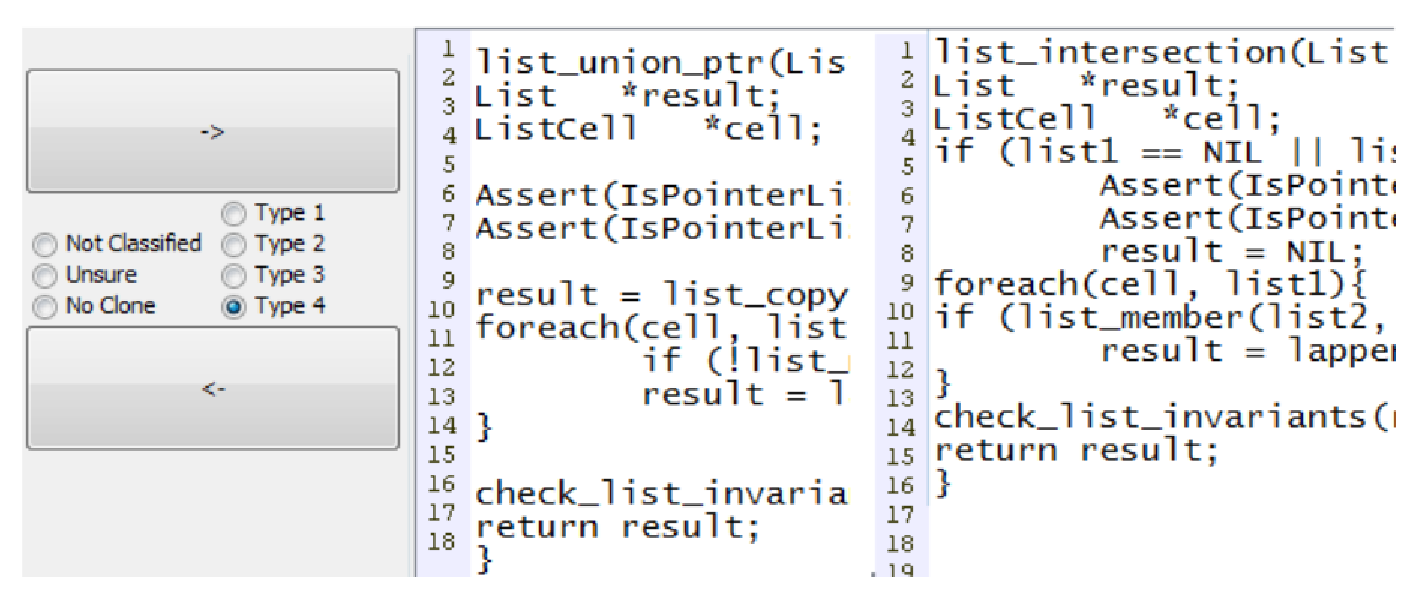
\includegraphics[width=\columnwidth, angle = 0]{tool.eps}
\caption{the {\it CloneInspection} tool}
\label{fig:clonediff}
\end{figure}


\section{Clones Discovered}
In this section, we first report the number of code clones discovered in this study and their types. We then provide an explanation on how the data available on our website should be interpreted.

\subsection{Clones and Their Types}

In Table~\ref{table:clonesfound} under {\it Expert}, we show the number of clones and clone types where the expert group makes consensuses. Under {\it Student}, we show the number of function pairs that at least half of the students identified as clones. Under {\it Agree}, we list the number where the experts and 50\% or above students agree they are clones.


As shown in Table~\ref{table:clonesfound}, we discovered clones from all of the three programs. We found 66 pairs of clones, 4.3\% of the total of 1536 function pairs examined. The majority clones found are type-2; however, we also find a total of 9 type-4 clones. No type-1 clones were noted, which is not surprising since developers can usually recognize exact duplications of code and would have removed them from the software.

Under {\it Student}, we show that individual students disagree significantly on what is a clone. If we increase the threshold from 50\% to 75\% and report a clone if 75\% students agree, we would see much less clones identified by the students. Under {\it Agree}, we see that the students agreed with 12 out of 15 pairs in {\it Python} and 33 out of 33 pairs in {\it PostgreSQL}, but only 7 of the 18 clones in {\it Apache}. Interestingly, {\it Python} and {\it PostgreSQL} contain type-3 and type-4 while {\it Apache} only contains type-2 clones, which typically are considered easier to confirm compared to type-3 and type-4 clones.

\begin{table}[thb!]
\begin{center}
\caption{Clones Identified in Oracle}
\vspace{0.1in} % Add a small buffer between title and table
\label{table:clonesfound}
\resizebox{\columnwidth}{!}{
\begin{tabular}{|r||l|l|l|l|}
\hline
\bfseries Application & \bfseries Clone & \bfseries Expert & \bfseries Student & \bfseries Agree \\ \hline\hline
  \bfseries Apache & \bfseries  T1 & 0 &  &\\ \cline{2-3}
   & \bfseries T2 &  18 && \\ \cline{2-3}
& \bfseries  T3 &  0 & & \\ \cline{2-3}
& \bfseries  T4 &  0 & & \\ \cline{2-5}
& \bfseries Total &  18 & 23 & 7  \\ \cline{2-5}
& \bfseries Not Clone &  339 & 334 & 303 \\ \cline{2-5}

\hline
  \bfseries Python & \bfseries T1 & 0 & & \\ \cline{2-3}
   & \bfseries T2 &  7 & &\\ \cline{2-3}
& \bfseries  T3 &  4 &  &\\ \cline{2-3}
& \bfseries  T4 &  4 &  &\\ \cline{2-5}
& \bfseries Total &  15 & 34 & 12 \\ \cline{2-5}
& \bfseries Not Clone &  530 & 522 & 473 \\ \cline{2-5}
\hline

  \bfseries PostgreSQL & \bfseries T1 & 0 & &  \\ \cline{2-3}
   & \bfseries T2 &  18 & &\\ \cline{2-3}
& \bfseries  T3 &  10 &  &\\ \cline{2-3}
& \bfseries  T4 &  5 &  &\\ \cline{2-5}
& \bfseries Total &  33 & 107 & 33 \\ \cline{2-5}
& \bfseries Not Clone &  601 & 550 & 459 \\ \cline{2-5}
\hline \hline
 \bfseries Total & \bfseries Clone & 66 & 164 & 46 \\ \cline{2-5}
  \bfseries  & \bfseries Not Clone & 1470 & 1406 & 1208 \\ \cline{2-5}

  \hline

\end{tabular}
}
\end{center}

%\vspace{-0.3in}
\end{table}

In Table~\ref{clone}, we display an example of a type-4 clone in {\it PostgreSQL} reported by an expert group and also classified by 50\% of the students as a clone. The code segments both implement the union of the two lists. The two segments use different function names and invoked different calls, e.g., {\it list\_member\_ptr} in the first segment, and {\it list\_member} in the second segment. The majority statements in the two functions are different. None of the existing code clone detection tools reported it as a clone.

\noindent
\begin{table*}
\caption{An Example of Type-4 Clones from PostgreSQL~\label{clone}}
\vspace{2 mm}
\begin{tabular}{c | c}
\bfseries Code Segment \#1  & \bfseries Code Segment \#2 \\ \hline \hline
\begin{lstlisting}
list_union_ptr(List *list1,List *list2)
	List   *result;
	ListCell   *cell;

	Assert(IsPointerList(list1));
	Assert(IsPointerList(list2));

	result = list_copy(list1);
	foreach(cell, list2){
		if(!list_member_ptr(result,lfirst(cell)))
			result=lappend(result,lfirst(cell));
		}
	check_list_invariants(result);
	return result;
}
\end{lstlisting}
&
\begin{lstlisting}

list_intersection(List *list1, List *list2)
	List   *result;
	ListCell   *cell;
	if (list1 == NIL || list2 == NIL)
		return NIL;

	Assert(IsPointerList(list1));
	Assert(IsPointerList(list2));

	result = NIL;
	foreach(cell, list1){
		if(list_member(list2,lfirst(cell)))
			result=lappend(result,lfirst(cell));
	}
	check_list_invariants(result);
	return result;
}
\end{lstlisting}

\end{tabular}
%\dan{I added indents to the code and cleaned things up in this table}
\end{table*}

\subsection{Data Available on the Project Website}
Both our tool and data are available on our website\footnote{\url{http://phd.gccis.rit.edu/weile/data/cloneoracle/}} in several formats including html, csv, xml and xls. Table~\ref{table:exampleoutput} shows an example of the publicly available data. Under {\it Comparison}, we list function pairs under study. The {\it Expert} column displays the type of clone agreed upon by the experts and a {\it No} if a clone was not found. The {\it Student} column shows the percentage of students who determined the pair is a clone. Finally, columns {\it Tool 1} and {\it Tool 2} report whether a specific tool determines if the pair is a clone. The table includes the results for all the 45,109 function pairs collected. Since only a subset of function pairs are selected for manual studies, the function pairs  not included in the manual studies are left blank under {\it Expert} and {\it Student}.  In addition to the detailed results shown in Table~\ref{table:exampleoutput}, we also report 66 pairs of code clones on the website. This value is sufficient since most previous works have only used 4-20 clones in evaluating clone detection tools~\cite{Roy:2009:CEC:1530898.1531101,Kraw2012}

% Krawitz - 4
% Roy - 16 ? // check this
% Detecting Code Clones in Binary Executables:
% Software Clone Detection:
% Comparision and Evaluation:
% COmparision and Evaluation:


\begin{table}[thb!]
\begin{center}
\caption{Example Results Output}
\label{table:exampleoutput}
\resizebox{\columnwidth}{!}{
    \begin{tabular}{ |l | l | l | l | l|  }
    \hline
%    \toprule
   \bfseries Comparison &\bfseries Expert & \bfseries Student & \bfseries Tool 1 & \bfseries Tool 2 \\ \hline \hline
   \bfseries MethA-MethB  & Type-1 & 100 \% & No   & Yes  \\ \hline
\bfseries MethB-MethC &  &  & No   & No  \\ \hline
\bfseries MethA-MethB & Type-3 &  75 \%  & Yes   & Yes   \\ \hline
\bfseries MethD-MethE & No &  0  & No   & No   \\
\hline
    \end{tabular}
    }
\end{center}

%\vspace{-0.3in}
\end{table}

\section{Limitations of the Data}

% Although we reported the data agreed by a group of experts and applied a wide variety of leading clone detection tools to help guide our decision making process,
Although our decision making process was guided in a variety of ways, there may be clones in our dataset that are not actually code clones, as manually determining code clones is not a trivial task~\cite{Walenstein:2003:PCT:950792.951349}.

The oracle we created only identified clones at the method level. While many clone detection tools are capable of only identifying clones at the method level, others may find them at a more granular level~\cite{Roy:2009:CEC:1530898.1531101}. Work may be done to create an oracle at the sub-method level.

In our studies, we did not find type-1 clones in the real-world code. However, such data are easily generated by adding white space and comments in the code and changing the code layout. On the other hand, type-1 clones can be determined by a compiler parser, and it is the types 2-4 clones that are valuable in the code clone oracle.

Finally, our oracle is C-based, meaning that the it will be of no use to clone detection tools which analyze code of other languages. Our technique is still very useful since a large portion of existing detection tools are C-based~\cite{Roy:2009:CEC:1530898.1531101}. We can extend our methodology to create oracles for other languages in the future.


\section{Related Work}
\label{sec: relatedworks}

Existing code clone data either are produced using only one tool, contain a small number of code clones, or do not include real-world type-4 clones. Our data set is produced with the considerations of a diverse set of clone detection tools and manual analysis, and thus have a higher confidence level. In addition, we studied over 1000 function pairs and produced 66 pairs of clones, including real-world type-4 clones, and thus our data set is also more complete.

Krawitz~\cite{Kraw2012} and Roy~\emph{et al.}~\cite{Roy:2009:CEC:1530898.1531101} both explicitly defined clones of all four types in a small controlled environment. However, these works only specified a small number of clones which were artificially created. In 2002, Bailey and Burd~\cite{Burd:2002:ECD:827253.827745} formed a manually verified clone data set which was used to compare three of the leading clone techniques at the time. This data has been criticized due to its validation subjectivity and its relatively small size. Bellon~\emph{et al.}~\cite{4288192} compared a set of code clone detection tools using a single researcher to manually verify the clones, but never publicly released all the discovered code clones~\cite{Roy:2009:CEC:1530898.1531101}.

Li et al.~\cite{Li:2012:CCB:2337223.2337260} and Saebjornsen~\emph{et al.}~\cite{Saebjornsen:2009:DCC:1572272.1572287} created a clone data set using clones identified by software developers. However, it is possible that developers only reported a small portion of the clones in the system since manually identifying code clones in a real world software system without the assistance of a tool is an extremely difficult and imprecise process. Lavoie and Merlo~\cite{Lavoie:2011:ATC:1985404.1985411} described an automated technique of constructing a clone data set based on the Levenshtein metric. While this is a powerful, automated technique for producing clones in large data sets, this is the only process used to create the oracle and but does not generate any verified data. Their approaches do not handle type-4 clones.

\section{Conclusions}
\label{sec: conclusion}
Code clone detection is important for bug finding, fixes and code search. In this paper, we describe the methodology and data for a code clone oracle which may be used by future researchers. The data are agreed by a group of experts with an assistant of a set of leading code detection tools. The 66 pairs of discovered code clones, the experimental data and tool are available on our website http://phd.gccis.rit.edu/weile/data/cloneoracle/.

%\section{Acknowledgements}
%We thank Luke Coy, Adam Blaine, Casey Klimkowsky, Shannon Trudeau and Steve~O~Hernandez for helping inspect code clones.

\bibliographystyle{abbrv}
\bibliography{cloneoracle}

% That's all folks!
\end{document}


%todo:
% Check on how the captions and labels should be (top or bottom)
%		- Table labels should go on top -  http://www.acm.org/sigs/publications/sig-alternate.pdf

% Information

% http://2014.msrconf.org
% 4 pages


%They are expected to be at most 4 pages long and should address the following: description of the data, % including its source; methodology used to gather it; description of the schema used to store it, and any limitations and/or challenges of this data set.

% Cit all the same, IE no 10,9 , [10][9] -> should be [3,8,10]



% Is it ok to include the source code of the applications on the project website (Apache, Python, Postgre)
%   At the very least, provide a link to download the specific versions from the actual project websites on the webpage.


